\subsection{The recoverability map on PTB-XL}
We estimate $\bm M_s$ (rank 3; the cardiac dipole is 3-D \emph{a priori}, and the cumulative
explained variance confirms rank~3 captures the bulk---a rank-sensitivity sweep $r{=}2\dots5$ is
reported in \texttt{results/recoverability\_maps.json}) per segment on the training NORM records,
with RECORD-LEVEL bootstrap CIs (resample records, refit $\bm M_s$; $\varrho{=}10^{-2}$;
Fig.~\ref{fig:map}). We plot the \emph{normalized} identifiability
$\tilde\eta_{s,\ell}=\eta_{s,\ell}/\|\bm e_\ell^\top\bm M_s\|_2$---a dimensionless relative
unobserved geometric gain (a ratio of $L_2$ norms, not a variance fraction). A single observed
lead leaves every other lead unidentifiable; a dipole-spanning $\{$I,II,V2$\}$ or
$\{$I,II,V1,V3,V5$\}$ makes all targets \emph{exactly} identifiable ($\eta{=}0$).

\textbf{The robust flagship is exact.} The six limb leads are exact linear combinations of I and
II, so $\bm M_{s,S}$ for limb-6 has \emph{exact} rank 2: precordial ST is \emph{exactly}
non-identifiable from limb leads at any SNR, independent of $\varrho$ (Prop.~\ref{thm:perlead}).

\textbf{Graded ordering: stable for QRS, weighting-sensitive for ST/T.} A duplicated-limb
sensitivity analysis (\texttt{results/lead\_weighting.json}: refit on the 8 algebraically
independent leads, on the \emph{same} records) shows the V1--V6 $\tilde\eta$ ordering is
bootstrap-stable for QRS (Spearman $\LWspearQRS$, CI lower bound $\LWspearQRSlo$;
anterior-before-lateral in $\LWantlatQRS$ of resamples) but \emph{not} robust for the
low-amplitude ST/T segments (ST Spearman point $\LWspearST$ with a wide bootstrap CI;
anterior-before-lateral in only $\LWantlatST$ of resamples). We therefore report the ST/T
$\tilde\eta$/ambiguity magnitudes with this caveat and \emph{do not} claim a fine ST/T ordering;
the binary limb$\to$precordial verdict above is the robust ST statement. The estimated subspace
also depends on diagnosis (a NORM vs.\ MI principal-angle sensitivity is reported), so the map is
a \emph{NORM-trained reference}.

\begin{figure}[t]
  \centering
  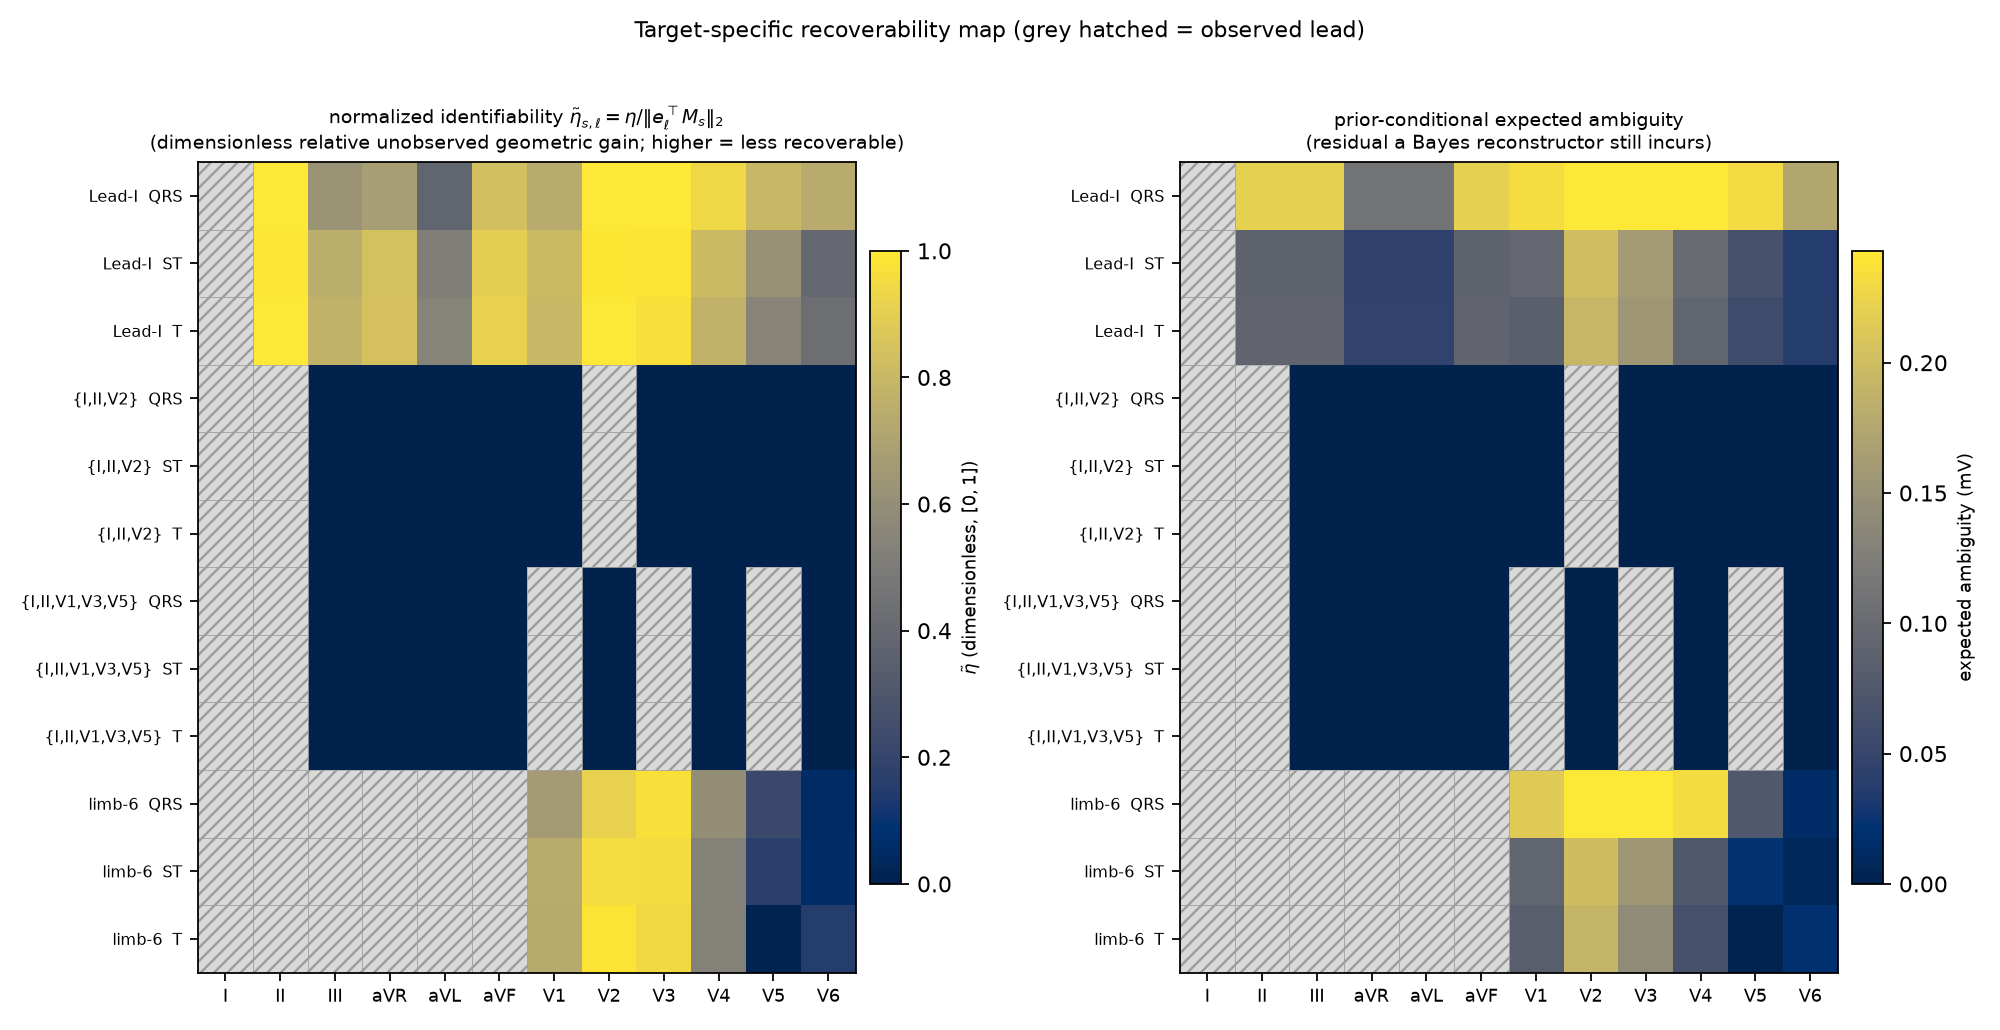
\includegraphics[width=\linewidth]{../results/recoverability_map.png}
  \caption{Recoverability map: normalized identifiability $\tilde\eta_{s,\ell}(S)$ (left,
  dimensionless) and prior-conditional expected ambiguity in mV (right), colorblind-safe
  \texttt{cividis}; grey hatched = observed. For limb-6 all precordial leads are unidentifiable
  ($\eta{>}0$); the fine ST/T ordering is weighting-sensitive (text).}
  \label{fig:map}
\end{figure}

\textbf{Downstream ST cost across reconstructors.} We reconstruct the full 10-second waveform
with three real continuous linear reconstructors (observed leads exact; ST at J$+$60\,ms vs.\ the
isoelectric PR-segment baseline [P offset\,--\,QRS onset], on fiducials from the observed Lead~II
shared between truth and reconstruction; median over beats; the PR-segment baseline fell back to
the pre-QRS window in $\approx\SafetyFallbackPct$\% of beats), and count ST-threshold events ($|$ST$|{\ge}0.1$\,mV; false positive =
crossing in reconstruction not truth, false negative = vice versa; Table~\ref{tab:safety}). On
$\SafetyN$ common records the \emph{total} wrong-event rate has point estimates ranging
$\TotWrongLo$--$\TotWrongHi\%$ across reconstructors and is \emph{dominated by false negatives}
(missed true crossings: limb$\to$precordial recovery smooths ST toward the population), with the
false-positive/false-negative split a reconstructor choice (paired record-bootstrap $\Delta$ on the
FP/FN split, and on the total, in \texttt{results/st\_safety.json}). We do not derive a minimax/Bayes
bound and make no equivalence claim: we report the range of total-error point estimates,
\emph{not} a certified lower bound, and ST-threshold events, not diagnoses. Because the PR-segment
baseline fell back to the pre-QRS window in $\approx\SafetyFallbackPct$\% of beats, the exact ST
magnitudes inherit that delineation limitation.

\begin{table}[t]
\centering\small
\caption{Limb-6 $\to$ precordial (all V1--V6) ST reconstruction, $\SafetyN$ common fold-10
records. FP/FN = false-positive/false-negative ST-threshold crossings (\%); total = FP+FN. FN
dominates (missed crossings); the split is a reconstructor choice. Auto-generated from
\texttt{results/st\_safety.json}.}
\label{tab:safety}
\begin{tabular}{lcccc}
\toprule
reconstructor & FP\,\% & FN\,\% & total\,\% & $|$ST$|$ err (mV) \\
\midrule
dipolar & \FpDipolar & \FnDipolar & \TotDipolar & \ErrDipolar \\
ridge   & \FpRidge   & \FnRidge   & \TotRidge   & \ErrRidge \\
OLS     & \FpOls     & \FnOls     & \TotOls     & \ErrOls \\
\bottomrule
\end{tabular}
\end{table}

\textbf{Truncation-tolerance sensitivity.} Well-posed configurations are $\varrho$-stable
($\{$I,II,V1,V3,V5$\}$ is rank~3 across $\varrho\!\in\!\{10^{-4},\dots,10^{-1}\}$); near-rank
-deficient sets are $\varrho$-sensitive and reported with the $\varrho$-sweep and bootstrap CIs.
A tiny-but-nonzero singular value is exactly identifiable yet $\varrho$-unidentifiable, which is
why we separate exact from $\varrho$-identifiability (Prop.~\ref{thm:perlead}).